\section{Static analysis framework}
\label{sec:frame}

\ToolP leverages a database-aware static analysis framework for 
Rails applications that we briefly describe below.

\subsection{Action dependency graph}
\ToolP's static analysis centers around the
action-dependency graph (ADG) that is constructed for each controller action.
Figure \ref{fig:icq} shows an example of ADG.

%As discussed in previous work \cite{powerstation}, 
An ADG is a database-aware extension 
of the traditional program-dependence graph (PDG)~\cite{ferrante1987program}.
Every node $n$ in the ADG represents an intermediate representation (IR)
statement in the corresponding action's JRuby \cite{jruby} IR.
Every edge $e$
represents either control dependency or data dependency. Edges shown in 
Figure~\ref{fig:icq} all represent data dependencies.

In contrast to the PDG, 
every node in the ADG that issues a SQL query is associated with a query tag in ADG, such as
node {\large \textcircled{\small 1}} and node {\large \textcircled{\small 2}} in Figure~\ref{fig:icq}. 
Information about SQL queries that are issued and the tables they referenced are determined by analyzing  {\tt ActiveRecord} function calls and recorded in the ADG.
%every query that might be issued by an IR statement is split out to be a special query-node in the graph, annotated with database table and fields accessed by the query.
%Furthermore, a data-dependency
%edge $n_1 \rightarrow n_2$ indicates that the output object $o$ of $n_1$ is used by $n_2$ without
%other statements overwriting $o$ in between. For each statement, we keep the line number information. Combining with the APIs provided by ActiveRecord and the database schema information, we further decide whether a node is a query. 
%This information is generated by carefully processing every model class extending the Rails
%{\tt ActiveRecord} interface, the {\tt schema.rb} file, invocations of {\tt ActiveRecord} query
%APIs, and others. 


Since view files may also contain Ruby code to process or render data, %contain computation and queries, and refer to Ruby variables, 
they are also analyzed during the ADG construction. Specifically, for every action, like
{\tt user/show} in Figure \ref{fig:icq}, its corresponding view file is identified based on an 
explicit {\tt render} statement or implicit file-name matching (as in
Figure~\ref{fig:icq}). The corresponding view file is then parsed, with all Ruby code embedded
inside {\tt <\% ...\%>} extracted and inlined as part of the ADG,
%appended to the action ADG 
%\cong{why ``append''? Might it do some other things after render? Maybe just say ``inline''}, 
like the three statements
inside {\tt show.html.erb} and the ADG shown in Figure \ref{fig:icq}. 

\begin{figure}
    \centering
    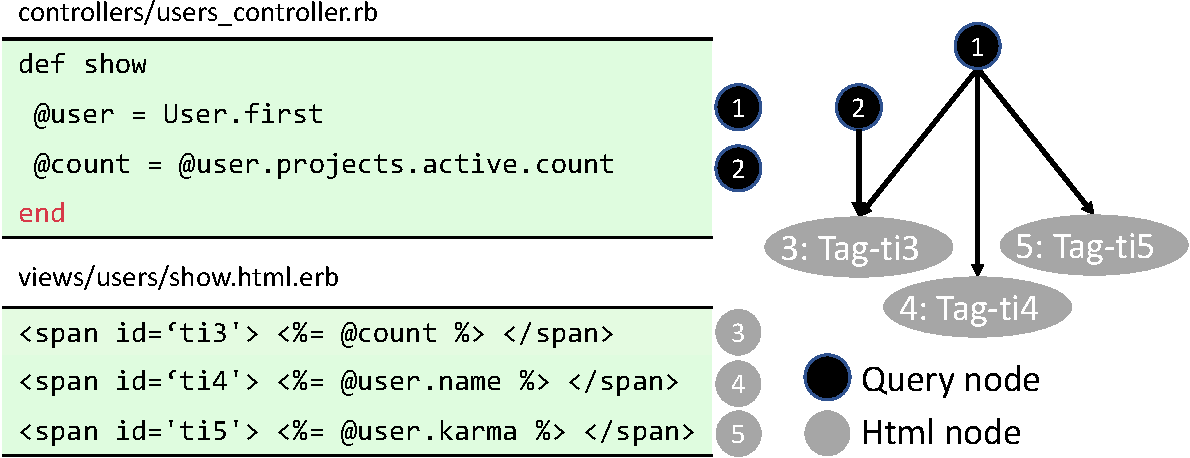
\includegraphics[width=0.7\columnwidth]{panorama-figs/code-example.pdf}
    \vspace{0.1in}
    \caption{Excerpt of an Action Dependency Graph}
    \label{fig:icq}
    \vspace{-0.2in}
\end{figure}

\subsection{Annotating the view component}
\label{sec:annotateview}
%\ToolP makes a few extension to the ADG generated by previous work 
%\cite{powerstation.fse18} for its view-centric analysis.
In order for \ToolP to attribute performance data correctly to each HTML tag,
\ToolP pre-processes every view file in the input web application
to assign every HTML tag a unique ID.
%through the HTML DOM (Document Object Mode). 
That is, for every tag {\tt <tag>} that does not already have an ID, 
\ToolP turns it into 
{\tt <tag id = ti>}, where {\tt ti} is a unique ID, as shown in the {\tt <span>} tags 
of Figure \ref{fig:icq}.
The current prototype of \ToolP does not handle HTML tags that are 
programmatically generated by JavaScript code.

%Next, while constructing the ADG, for every node coming from a view file, 
As mentioned, the view file has Ruby code embedded within it. For every node in ADG whose source code is in a view file,
\ToolP identifies its inner-most surrounding HTML tag and associates it with the corresponding tag ID.
\ToolP also %parses the view file to see 
checks whether its corresponding content is rendered or not by analyzing the HTML, and
assigns an {\tt is\_rendered} property accordingly. 
This information will help \ToolP attribute data processing cost to each HTML element and identify alternative view designs, as we will explain in later sections.
%\cong{Why is this necessary?}


%%%%%%% COMMENT OUT %%%%%%
\iffalse
The PDG generated above is then extended in three ways to create the ADG: 
(1) changing and splitting some nodes to become 
Query nodes; (2) annotating every Query node with the database table and fields that are read or written; 
(3) annotating every outgoing data-dependency edge of a Query node with the exact field(s) that are used.


To accomplish this, previous work first analyzes every model class that extends the Rails
{\tt ActiveRecord} interface to determine all the database
tables in the application and the association relationship among them.
For example, analyzing the model classes illustrated in 
Figure~\ref{fig:schema}, \ToolP identifies the {\tt users} table
corresponding to the {\tt User} class and similarly for the {\tt Blog} class, and that these two models have 
a one-to-many relationship, i.e., each instance of {\tt User} may own multiple instances of {\tt Blog}.
Second, \ToolP analyzes the {\tt schema.rb} file to determine
how many fields each table contains. For example, parsing the
{\tt schema.rb} snippet in Figure~\ref{fig:schema}, \ToolP learns about 
the schemas of table {\tt users} and {\tt blogs} as
shown in the bottom of the figure.

Third, \ToolP identifies queries from three sources: (1) explicit 
invocations of
Rails {\tt ActiveRecord} Query APIs, such as {\tt exist?},
{\tt reload}, \textit{\tt update}, \textit{\tt destroy}, etc;
(2) implicit queries generated by Rails to access object fields, e.g., {\tt $o_1$.$o_2$}, where 
the class of $o_1$ and the class of $o_2$ are associated model classes
(e.g., {\tt user.blogs} would incur a query to
retrieve records in {\tt blogs} table that are associated with
the specific {\tt user} record in {\tt users} table);
(3) explicitly invoked raw SQL queries through  Base.connection.execute.
%\junwen{it's also thru the ActiveRecord API, similar as the first type}
Any query identified above is represented as a Query node in the ADG.\footnote{At run time,
multiple such queries could be composed by ORM into one SQL query.
Such query chaining does not affect \ToolP analysis.}
\fi